\documentclass[tikz, margin=2mm]{standalone}

\begin{document}
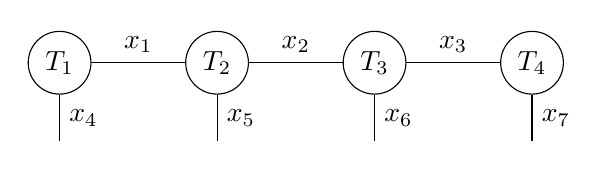
\begin{tikzpicture}
    \node[circle, draw] (T1) at (0,0) {$T_1$};
    \node[circle, draw] (T2) at (2,0) {$T_2$};
    \node[circle, draw] (T3) at (4,0) {$T_3$};
    \node[circle, draw] (T4) at (6,0) {$T_4$};

    \draw (T1) -- node[above]{$x_1$} (T2);
    \draw (T2) -- node[above]{$x_2$} (T3);
    \draw (T3) -- node[above]{$x_3$} (T4);

    \draw (T1) -- ++(0,-1) node[midway, right]{$x_4$};
    \draw (T2) -- ++(0,-1) node[midway, right]{$x_5$};
    \draw (T3) -- ++(0,-1) node[midway, right]{$x_6$};
    \draw (T4) -- ++(0,-1) node[midway, right]{$x_7$};
\end{tikzpicture}
\end{document}